% !TEX root = SocialVision2014.tex
\vspace{-5pt}
%\subsection{Datasets and challenge problems}
\subsection{Data, evaluation, and challenge problems}
\label{sec:sys}
\vspace{-5pt}

An encouraging recent trend has been the increasing use of benchmark datasets for evaluating progress on particular tasks. Standardized dataset \comment{such as the Middlebury Stereo Evaluation project~\cite{ScharsteinS02} and the PASCAL VOC Challenges~\cite{Everingham10}} have served as catalysts for progress on difficult problems because they create concrete targets that inspire new ideas and allow to evaluate systems by quantitatively demonstrating improvement. As part of the proposed activity, we will build and share analogous benchmarks and challenge problems for interaction analysis and visual social network analysis, in addition to for enabling our own progress, to engage our colleagues. We will create at least four datasets, two based on images and two based on videos.


\comment{ in diverse, unconstrained environments. These benchmarks will serve as good proxies for real-world applications like analyzing online photo collections that can be pre-processed with face and body detectors, and analyzing videos from networked camera arrays and surveillance networks (e.g.,~\cite{CamNetRoy}) that can be pre-processed by (multi-view) detection and tracking systems (e.g.,~\cite{EshelM10,CamNetSclaroff}). These scenarios are fundamentally different from those considered in existing datasets for interaction analysis~\cite{UTdata,Choi:recogtrack,Patron-PerezMRZ12}, where the interactions are only weakly socially-relevant; involve a pre-determined number of participants; occur in the absence of non-participating by-standers; and/or are localized \emph{a priori} in space and time. We will create fundamentally different benchmarks and challenge problems that move beyond these limitations and provide better proxies for progress on real-world problems.} 

\boldstart{Image-based benchmarks}. We will harvest one of our image-based benchmark from personal photo albums embedded in a real social network, such as Facebook, using techniques established by PI Zickler~\cite{Stone2008,Stone2010,PintoZickler2011}. This image corpus will be annotated with body poses, identities, and metadata about the social relationships of co-occurring individuals, thereby enabling the quantitative evaluation of methods for learning and detecting static proxemes, like those in Fig.~\ref{fig:prodic}(b), as well as methods for inferring social relationships and networks. \comment{Some aspects of this data, such as the anonymized per-image coordinates of facial and body key-point locations, will be made publicly available to other researchers through the PIs' websites, while sensitive identity and social relationship information will be maintained securely at Harvard University and made available to researchers through secure collaboration mechanisms that are designed in consultation with the Institutional Review Board. PI Zickler has  been successfully using such a secure collaboration process for the classroom videos described below, and it works by having external collaborators: 1) trained in the ethics of research on human subjects through an online course; 2) approved as collaborators by the Institutional Review Board; and 3) conduct their research through remote connections to VPN-protected servers that are maintained by Harvard University.} A second \comment{completely public} image-based benchmark dataset will be created by collecting and annotating publicly-available Internet images using keyword searches. These will be made publicly available through the PIs' websites, along with body pose annotations that enable evaluation of learning, detecting, and recognizing static proxemes. We will publish side-by-side comparisons of performance on the private and public datasets whenever algorithms can be evaluated on both. This is a strategy that PI Zickler has previously employed for research on private photo collections~\cite{PintoZickler2011}, and it means that any researcher who evaluates their algorithms on the all-public dataset can quickly obtain estimates of how well those same algorithms might perform in a real social environment.

\boldstart{Video-based benchmarks}. We will create a video-based benchmark dataset, called the \emph{Harvard Interactive Classroom Dataset}, by leveraging video that has been collected by a six-camera array in a large classroom at Harvard University. This system has been developed by PI Zickler over the past few years with funding by the NSF (IIS-0835338, 2009--2012) and the Harvard Initiative for Learning and Teaching (HILT)\footnote{\href{http://hilt.harvard.edu/2012-2013-awards}{http://hilt.harvard.edu/2012-2013-awards}} with the goal of understanding how students learn in interactive classrooms, and a preliminary version of this data has already been used by the PIs~\cite{groupdet2013}. The observed classroom is ``interactive'' because students frequently engage in the process of \emph{Peer Instruction}, which works as follows. The process begins with a single ConcepTest---a question designed to elicit common student misconceptions~\cite{Crouch:PI,Mazur:PI}---and the students are given a moment to quietly formulate and electronically submit their individual answers. Then they are asked to form ad-hoc discussion groups to try to convince neighboring students of the correctness of their answers. After a few minutes of peer-to-peer discussion, students submit their possibly-revised answers, and this entire activity is followed by the instructor's reinforcement of the main concept. \comment{This process is repeated during the time normally devoted to lecture, and education research shows that both high- and low-ability students benefit~\cite{Fagen2002,Hake1998,Okebukola1984,Peterson1979}.}

The videos collected by this system present an extraordinary opportunity for developing and evaluating social visual analysis. The observed classroom---crops from which are shown in Fig.~\ref{fig:prodic}(a)---contains a hundred or more individuals engaged in ad-hoc interactions, and this creates a social environment that is fundamentally different from other benchmark datasets. The utility of this data stems not only from the number and diversity of people it contains, but also from the nature of the interactions, the duration of the observations, and the non-visual sources of metadata available for validation (e.g., audio recordings from 48 microphones; educational outcomes; answers to ConcepTests and exams; gender; age; and ethnicity). The original videos were collected over three months (about 200 camera-hours) and include more than fifty Peer Instruction sessions lasting a few minutes each and involving dozens of small-group discussions.

\comment{
As described in~\cite{groupdet2013}, we have already begun developing a suite of image analytical tools for ``pre-processing'' the classroom videos using implementations of face detection and tracking, identity recognition, and head pose estimation that together provide time-varying individual and pairwise descriptors ($\mathbf{f}$ and $\mathbf{g}$ in Sec.~\ref{sec:activity}). These descriptors are affected by many sources of noise---false detections, missed detections, uncertain identities, uncertain pose---and are therefore good proxies for many real-world environments. We will continue developing this pre-processing suite during the award period to extract richer head and body descriptors, such as histograms of flow, space-time interest points, and other features that capture elements of pose, motion, and gestures.

Under supervision by our Institutional Review Board, the classroom videos were recorded with consent from students and instructors and then stored and analyzed on VPN-protected servers. More than 95\% of the observed students provided consent for their videos to appear in academic publications and presentations, allowing disseminate of results through regular academic channels. We will engage external research groups with this dataset in three different ways. First, we will welcome collaborators to analyze the raw data on our VPN-protected servers using the secure protocol described above for images. Second, once we have developed low-level visual descriptors with satisfactory quality, we will anonymize and share these time-varying descriptors as proxies to the original imagery. Third, we will make use of advancing technologies for privacy-preserving social science research---like those currently being developed by colleagues at Harvard University\footnote{\href{http://privacytools.seas.harvard.edu}{http://privacytools.seas.harvard.edu}}---to enable more direct sharing of data.
}

A second\comment{completely-public} video-based benchmark dataset will be created by annotating identities, and face and body landmarks, in appropriate frames across multiple episodes of a serial television show, such as \emph{The Wire},\footnote{\href{http://www.hbo.com/the-wire}{http://www.hbo.com/the-wire}} that involves an elaborate social network. To adhere to copyright policies, we will publicly share only the annotations for the television show, and not the raw video data. These annotations should be sufficient on their own for benchmarking all of the tasks described above, and they will be time-indexed so that any researcher who desires can purchase their own copy of the raw video and accurately superimpose our annotations.






%%%%%%%%%%%%%%%%%%%%

%\boldstart{Facebook Photo Dataset}\cite{Stone2008}. The Facebook Photo Dataset was collected from 53 volunteers of active Facebook community members, who agreed to contribute photos and metadata through a web API. Using the API, all photos posted by each volunteer, all photos tagged with any of our volunteers� Facebook friends, all tags associated with any of these photos, and the network of friendships among our volunteers and their friends were archived. A total of 1.28 million tagged photos were retrieved, and all volunteers and tagged friends number 15,752 individuals in all. From this collection, PI Zickler and other collaborators automatically detected and aligned 438,489 face samples that could be associated with the identity labels manually entered by the volunteers. The Facebook dataset was used as the first type of face dataset with social context and enabled the first ``socially-aware" face recognition system \cite{Stone2008}.

%In our proposed research, we will retrieve a new photo collection from appropriate online social platforms, and solve the inverse problem: obtaining social network from images. We will inherit the successful data collecting scheme in \cite{Stone2008} by deploying web-based API to volunteers' account, but the new photo collection will be different from the previous dataset in the following aspects. First, we will look into more appropriate online social platforms that emphasize on photo sharing, so that we may obtain more diverse imagery with richer visual cues, e.g.,bodies and scene contexts, than simply faces. Second, we will try to obtain richer annotations about social semantics as well as other metadata than just friendships, with the consent and help from the volunteers. Third, and most important, we will follow a similar strategy as used for the Harvard Interactive Classroom Dataset in producing an publishable version of this dataset, by allowing access to them through our privacy-preserved server, providing anonymized descriptors and metadata, or borrowing other advancing technologies from privacy-preserving social science research.


%\begin{figure}[t!]
%\begin{center}
%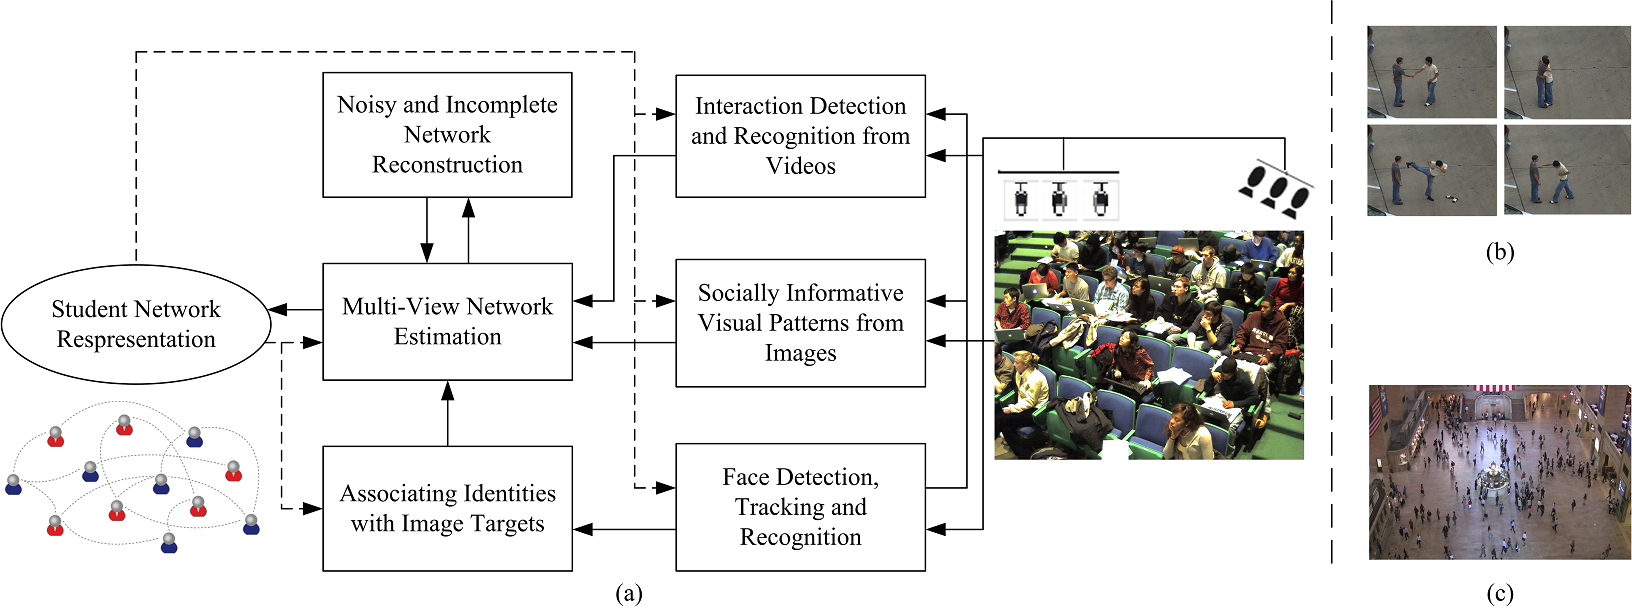
\includegraphics[width=\columnwidth]{prototype_1}
%\end{center}
%\vspace{-0.25in} \caption{\captionsize 
%Interactive classrooms are attractive research testbeds because unlike most existing datasets (b: \cite{UTdata}) they contain diverse behaviors in a real, cluttered environments, and therefore provide strong proxies for social visual analysis in the wild (c: \cite{WangMG09}). We will evaluate our research systems on videos collected from a classroom observation system (a) that already exists at Harvard University.}\label{fig:prototype}\end{figure}



%Our goal is to build a foundation for social analysis in diverse, unconstrained environments like Fig.~\ref{fig:prototype}(c). This is becoming well within reach due to increasing availability of networked camera arrays and advances in practical multi-view detection and tracking (e.g.,~\cite{EshelM10}). These unconstrained environments are fundamentally different from scenarios considered in most existing benchmark datasets for interaction analysis (Fig.~\ref{fig:prototype}(b)), where the interactions involve a pre-determined number of participants; take place in the absence of by-standers or social clutter; and/or are localized  \emph{a priori} in time~\cite{UTdata,Choi:context,Choi:recogtrack,CRIM13}. Because of these  differences, evaluations on existing benchmarks fail to provide meaningful proxies for fundamental progress in widespread social visual analysis.




%As part of the proposed activity, we will create new datasets and challenge problems that make it possible to measure meaningful progress on social visual analysis, and at the same time, serve as mechanisms to engage the broader research community. To ensure our benchmarks provide effective measures of progress, they will be annotated with ground-truth information about identities, interaction categories, and social relationships. We will create and use two distinct types of datasets. The first type will be based on video collections that are already being collected in interactive classrooms at Harvard University. These datasets will be large (more than 350 camera-hours so far) and will enable evaluation of all aspects of the proposed research program. Because of privacy restrictions they will not be made directly available to non-collaborating research groups, so we will create a second set of  datasets for this purpose.

%As part of the proposed activity, we will create new datasets that make it possible to measure meaningful progress on social visual analysis, and at the same time, serve as mechanisms to engage the broader research community, by enabling the evaluation of certain aspects of the proposed research program (e.g., detecting and recognizing proxemes). These will be presented as ``challenge problems" for the broader computer vision research community. 



%In the first image set there will be photos depicting co-occurrences of individuals in various social environments that are collected from internet by keyword search as those in Fig~\ref{flicker}, using which we will learn and detect socially informative proxemes\comment{from pairwise poses and other visual cues, but without estimating social networks}. The second image set will be personal photo albums from Facebook as used in~\cite{Stone2008,Stone2010,PintoZickler2011} where social network information is available, on which we will implement the entire framework introduced .in this proposal. 

%In companion, the first video set will be appropriate seasons and/or episodes of selected TV shows or movies (as shown in Fig.~\ref{fig:socialbehavior}(a)) in which a well-shaped social network exists among characters. Finally, the second video set will be the video collections that are already being collected in interactive classrooms at Harvard University and we will use it as a testbed for reconstructing a specialized social network consisting of class of students. These large-scale datasets will enable evaluation of all aspects of the proposed research program. 


%Because of copyright restrictions, we will make available the annotations for the TV-show/movie dataset but not the original videos, and interested researchers may directly purchase their copies of videos. Because of privacy restrictions, Facebook albums and Harvard Interactive Classroom Dataset may not be made directly available to non-collaborating research groups, and we will create their alternative sets or subsets that public can share. In the following, we provide more introduction to the Harvard Interactive Classroom Dataset that we have been collecting and preliminarily evaluated in \cite{groupdet2013} by the PIs, as well as the Facebook Photo Dataset \cite{Stone2008} by PI Zickler, which serves as a motivating prototype for the new Facebook dataset to be collected.


%Another useful property of the original video dataset comes from the many non-visual sources of metadata that are associated with it. First, for each Peer Instructions session, the dataset contains records of the students' answers to multiple-choice questions before and after their peer-to-peer discussions. Second, thanks to the immense past efforts of collaborating educational experts (funded by other sources and using qualitative analysis techniques like those in~\cite{Scherr2009}), a small number of semantically-meaningful behavioral units have been defined, and occurrences of these behavioral units have been painstakingly annotated in space and time. This means, for example, that when computer vision researchers develop new techniques to discover and detect large numbers of proxemes, they can compare them quantitatively with those identified by human experts. 


%In conjunction with our Institutional Review Board, the original classroom videos were recorded with consent from students and instructors, and were stored and analyzed on VPN-protected servers. More than 95\% of students provided consent for their videos to appear in academic publications and presentations, allowing researchers to disseminate their results through regular academic channels. This same consent extends to the subset of the original videos that appear in the Harvard Interactive Classroom Dataset. Researchers from a number of other institutions are already collaborating to analyze this data in a secure manner. Each collaboration happens by the external collaborator(s): 1) being trained in the ethics of research on human subjects through an online course; 2) being approved as collaborators by our Institutional Review Board; and 3) conducting their analysis through remote connections to our VPN-protected servers. These VPN-protected servers are being maintained by the Research Computing Group in the Faculty of Arts and Science at Harvard University, and they will continue to be maintained well beyond the end of the award period.







%In conjunction with our Institutional Review Board, we have established a protocol in which classroom videos are recorded with consent from students and instructors, and then stored and analyzed on VPN-protected servers. More than 95\% of students also provide consent for their videos to appear in academic publications and presentations, allowing us to disseminate our research results through regular academic channels. But since the classroom videos cannot be made directly available to research groups other than ours, we will promote reproducible research in three different ways. First, as described in the next section, we will create smaller parallel  datasets that are publicly-available and allow other research groups to evaluate algorithms for certain aspects of social visual analysis. Second, we will welcome interested research groups to collaborate with us to evaluate their algorithms on our classroom data by running their code on our VPN-protected servers. Third, whenever possible we will make use of advancing  technologies for privacy-preserving social science research---like those currently being developed by colleagues at Harvard University\footnote{\href{http://privacytools.seas.harvard.edu}{http://privacytools.seas.harvard.edu}}---to enable more direct sharing of classroom data for research purposes.

%\boldstart{Challenge problems}. An encouraging trend over the last several years has been the increasing use of benchmark datasets for evaluating progress on particular tasks. Standardized datasets, such as the Middlebury Stereo Evaluation project~\cite{ScharsteinS02}, the PASCAL VOC Challenges~\cite{Everingham10}, and the Hollywood database of individual actions~\cite{LaptevMSR08}, have served as catalysts for progress on difficult problems because they create concrete targets that inspire new ideas and allow researchers to evaluate their systems by quantitatively demonstrating improvement. Currently, there are relatively few datasets available for problems related to social visual analysis, and those that do exist consider severely constrained environments that are not good proxies for the real world.

%As part of the proposed activity, we will create new datasets and define challenge problems that engage the computer vision research community in our research agenda. These will be collections of annotated videos that contain interactions staged by informed actors, and they will simulate unconstrained environments by including long videos of large social gatherings. They will be annotated with identities, relationships, and interaction categories, and will thereby  enable the evaluation of certain aspects of the proposed research program (e.g., detecting interaction categories). These will be presented as ``challenge problems" for the broader computer vision research community. We will also publish side-by-side comparisons of our performance on these publicly-shared benchmarks and analogous, but larger, benchmarks derived from our private classroom data. This is a strategy that PI Zickler has previously employed for research on private photo collections~\cite{PintoZickler2011}, and it means that any researcher who evaluates their algorithms on the public datasets can obtain an estimate of how well those same algorithms might perform in a  real classroom environment.

%With this established classroom observation system and these fundamental modules, we have successfully collected and processed a large-scale classroom behavior database consisting of 100 video clips in total. The students are seated in a regular lecture hall and are observed by a camera array with non-overlapping fields of view. The classroom is ``interactive'' because at various times throughout the lecture students are invited to engage in ad-hoc group discussions about problems provided by the instructor. The scale of our database is orders of magnitude larger than state-of-the-art computer vision datasets (e.g. those used in \cite{UTdata,Choi:context,Choi:recogtrack}), in the number of individuals (10-50 students per camera), the number of cameras (6), and the amount of time (100 minutes per camera, per recording, equaling over 3,000 minutes in total). Through a combination of face detection and tracking, we obtained noisy tracks for all students in each monocular video, upon which we developed descriptive modules that directly extract descriptiors such as head pose and body motion, we have also implemented a high-level module for behavior analysis based on similarity between two social groups, as depicted in Fig. \ref{fig:prototype}(b). In this module, the behavior of each individual is represented by a combination of the head pose and the motion of torso and arms (using the method of histogram of optical flows). The social behavior of a group is then represented by the configuration in space and time of the behaviors of its participants. With this social activity representation, the module detects a salient social activity from a new video and retrieves similar social activities from our established database. This functionality is illustrated in Fig. \ref{fig:prototype}(b), where our system has discovered a three-way conversation by identifying the participants of this conversation and the time span (several to tens of seconds) of this event. Based on the behavior representation for this space-time social interaction, the system searches the remainder of the database and retrieves a list of exemplars containing similar social behavior, ranked in the descending order of the similarities with the query. In this way, any manual annotations associated with the query video can be propagated to the top-ranking exemplars, and we are now taking this approach to propagate our manual annotations across the whole database. 








%At the current and initial stage of the effort to bring socialized semantics to computer vision, it can be usually the case that we do not have sufficient social contexts to help improving our target/face recognition, and we are not always specific about what are the meaningful social interactive activities that are most informative for social description. Conversely, we may neither know clearly about what exactly we should distill from images to fulfill a network learning task, nor have concrete knowledge about how the multiple views or overlapping community structures of a network will eventually turn out to be. However, we have argued at the beginning and demonstrated through the four proposed research problems the fact that the two aspects assist and benefit from each other, and an overall socially-aware visual analytical system is our ultimate goal. To this end, our final proposed research will include an attempt for a framework that eventually integrate social information and image understanding and allow them to learn and self-build themselves in an evolving and unsupervised manner.





